\documentclass[11pt]{article}
\usepackage[T1]{fontenc}
\usepackage[utf8]{inputenc}
\usepackage[english]{babel}
\usepackage[colorlinks=true]{hyperref}
\usepackage{mathrsfs}
\usepackage{geometry}
\usepackage{fullpage}
\usepackage{listings}
\usepackage{xcolor,graphicx}
\usepackage{xspace}
\usepackage{verbatim}
\usepackage{textcomp}
\usepackage{amsmath}
\usepackage{amsfonts}
\usepackage{syntax}
\usepackage{amssymb}

\title{Query compilation in a functional web programming language}
\author{Gabriel \textsc{Radanne}\\ University of Edinburgh\\ Under the supervision of Sam Lindley, James Cheney and Philip Wadler.}
\date{\today}

\newcommand\mysc[1]{{\rmfamily\textsc{#1}}\xspace}
\newcommand\links{\mysc{Links}}
\newcommand\sql{\mysc{SQL}}
\newcommand\js{\mysc{Javascript}}
\newcommand\ocaml{\mysc{Ocaml}}

\newcommand\refsec[1]{\hyperref[#1]{section \ref*{#1}}}


\lstdefinelanguage{links}{
  morekeywords={var,for,where},
  otherkeywords={<-,<--,=},
  morekeywords=[2]{table,database,with,from},
  classoffset=0,
  morestring=[b]",
  morecomment=[s]{/*}{*/}
}


\lstset{
  tabsize=4,
  basicstyle=\ttfamily\scriptsize,
  % upquote=true,
  aboveskip={0.5\baselineskip},
  columns=fixed,
  showstringspaces=false,
  extendedchars=true,
  breaklines=true,
  prebreak = \raisebox{0ex}[0ex][0ex]{\ensuremath{\hookleftarrow}},
  showtabs=false,
  showspaces=false,
  showstringspaces=false,
  identifierstyle=,
  keywordstyle=\color[rgb]{0.1,0.1,0.7},
  keywordstyle=[2]\color[rgb]{0.1,0.6,0.1},
  commentstyle=\color[rgb]{0.5,0.5,0.5},
  stringstyle=\color[rgb]{0.727,0.326,0.2},
}

\newcommand\sig[1]{{\tt\bf #1}}
\newcommand\code[1]{{\tt #1}}
\newcommand\linkslst[1]{\lstinputlisting[language=links]{#1}}
\newcommand\effect[1]{{\em #1}}

\newcommand\ocamlc[1]{\lstinline[language={[Objective]Caml},basicstyle=\ttfamily\normalsize]{#1}}

\newcommand\module[1]{{\bf #1}}

%comment inside bnf
\renewcommand\comment[1]{{\color{gray} $//$ #1}}

\begin{document}

\begin{titlepage}
  \maketitle
  \thispagestyle{empty} % remove page number

\paragraph{Abstract}
  \links \cite{links:tiers} is a functional programming 
language for creating web applications. From a single source program 
\links produces \js for the client, \sql for database access, and 
an interpreted intermediate language for the server.

A prototype compiler to \ocaml has been done during a previous internship \cite{links:querycomp} but is missing support for queries. The goal of this project is to add the support to generate \sql query into this compiler. This is difficult because the query generation in \links is done by inspecting the syntax of the program at runtime \cite{links:querynorm}, syntax which is not available normally in the compiled code.

During this internship, the chosen approach, following \cite{links:querycomp},  was to apply a transformation to the program by duplicating each function: one will be compiled normally, the other one will be used to make the syntaxic information available in the compiled file.

\paragraph{Key-words} \sql, query, compilation, effects, functional programming.

\end{titlepage}



\section{A quick introduction to Links}

\subsection{What is Links ?}
In a nutshell, Links is a web functional programming language. We can define Links by two goals.

\links aims to avoid code separation between the client, the server and the database. In usual web programming, you keep these three components separated, for example: the client is written in \js, the server in \mysc{PHP} and queries are in \sql. 
This separation leads to what is called {\it the impedance mismatch} problem : How to be sure that the type of data received by the \sql Query, fits the server expectations?

One of the first \links' related article \cite{links:tiers} was called ``web programming without tiers'' : In \links, there is only one language for the client, the server and the queries. 
The strong type system ensures that data traveling between these three parts will properly work together. 
The language itself will decide if the function should be on the server or on the client side, ensuring data availability.

In \links, the client part is compiled in \js and the server part is interpreted.

Another goal of \links is to use the functional paradigm and a strong type system to ease web programming with useful abstractions. \cite{links:formlets} and \cite{links:effect} introduce new concepts such as the manipulation of form components and queries in a strongly typed way.\\

Apart from this web functionality, \links is a fully featured strongly typed functional language with algebraic datatypes, pattern matching, lambda abstraction and so on.\\

During a previous project \cite{links:comp}, a compiler for the server part as been done, but this compiler is incomplete since it does not handle queries. The goal of this internship is to allow queries in \links to be compiled.\\

The next section will present the query system of \links in more details.

\subsection{The Query system\label{intro:query}}

Queries in \links are integrated as an element of the language. As opposed to most server side languages, you does not write \sql strings : you just write the usual code and it will be translated into an \sql query during runtime.

As an example, here is a simple piece of \links code with a query: 
\linkslst{simplequery.links}
The first line is a database declaration. The details on how to connect to this database through the network is given by a configuration file.\\
Then a table is declared, with its type which must be some fields of basic types. Here it's only one field \code{``word''} of type \sig{String}.\newpage
After this declaration, a query is done, using a for comprehension with the long arrow \code{<-\--}. This query fetch everything from the table. This is exactly equivalent to the \sql code :\\ \verb+select * from hello+.\\
 Finally a proper for comprehension, with a short arrow \code{<-}, project the field \code{word} of every element of the result.\\
The output of our small program is a list of strings. With the proper table :
\begin{lstlisting}
["hello", "world", "!"] : [String]
\end{lstlisting}\ 

You can of course make more complex queries by using a where clause, an orderby clause or by applying treatment to the output.\\

Usually in \sql, the output of a query is a table, which is a list of rows where each row is made of named fields : the columns. Each field can only be a simple type like string, float, integer or boolean.\\
The natural translation in \links' typesystem is a list of records.\\

This tight integration between queries and the programming language has two consequences:
\begin{itemize}
\item The language must ensure than every function that appears inside a query can actually be translated. For example you cannot translate recursive functions to \sql.
\item Each function can have up to two meanings: a \effect{query} meaning and a \effect{language} meaning.
\end{itemize}

Effects, as described in \cite{links:effect}, allow \links' type system to handle that specificity nicely.\\

Effects can be described as a way to characterize what a function is doing during its computation. 

For example, let's look at the \code{print(s)} function. Its type is \sig{(String) -\{wild\}-> ()}. \sig{wild} is an effect which indicate that this function cannot be run in a query. This makes sense since \sql does not have a printing function.

Let's now look at the \code{curry(f)} function with the type \sig{((a, b) -c-> d) -> ((a) -> (b) -c-> d)}. If the function \code{f} passed to \code{curry} have an effect \sig{c}, the application of the curryfied function will also get this effect.\\

This will allow us to know if a function can be used inside a query or not.\newpage

Here is another example where a predicate function is used to filter the result of a query during the query, using \code{<-\--}, and after the query, using list processing.
\linkslst{querypredicat.links}\label{examplepred}
As in the previous example, we first declare a database and a table, with a field \code{i} of type \sig{Int} and e field \code{n} of type \sig{String}.
The \code{do_query} function take a predicate as an argument and compute two query
\begin{itemize}
\item The first one: \code{for (x <-- my_table) where (p(x.i)) [x]} will be translated to a query with a where clause, using the p function.
\item The second one: \code{for (t <-- my_table) [t]} is just fetching everything from the table. It will be filter \emph{as a list} by the next command.
\end{itemize}

Then, the function compares the two results. Of course, the result will always be \code{True}.

The signature of the \code{do_query} function is the following : \sig{fun : ((Int) \{\}-> Bool) \{\}-> Bool}. This function takes a predicate function that return a Boolean. The arrow \sig{\{\}->} means that we can not have any \sig{wild} effect here.

This example shows that this predicate function can be used in two way: as a regular function used in list processing or as a piece of syntax that can be translated to \sql.

\section{\links' insides}

\links' compiler and evaluator are implemented in \ocaml. 
The code can be separated into two parts. 
The front-end takes care of various static analysis including type inference and removing any syntactic sugar. 
At the end of this first stage, the code is in an internal representation defined in the \module{Ir} module and which will be presented in \refsec{ir}. 

Then the backend will transform this internal representation into different forms.\\
The client side code will be extracted from it and compile to \js by the \module{Irtojs} module.\\
The server side will be evaluated by the \module{Evalir} module or compiled to \ocaml by the \module{Irtoml} module that will be presented \refsec{irtoml}.\\
In case the server side is evaluated, the \module{Query} module handle the query normalization that will be explained \refsec{querynorm}.

\subsection{The internal representation \label{ir}}

The internal representation of \links is in ANF\footnote{A normal form}. This a representation of a program where every argument is trivial and does not need any computation to be evaluated. 

For example this program:
\begin{lstlisting}[language={[Objective]Caml}]
f(g(x),h(y))
\end{lstlisting}
Can be converted in ANF:
\begin{lstlisting}[language={[Objective]Caml}]
let x'=g(x) in
let y'=h(y) in
f(x',y')
\end{lstlisting}

ANF is a very simple representation that transforms usual complex transformations to very simple ones. It is also isomorphic to CPS\footnote{Continuation Passing Style}.\\

Here is a simplified representation of the internal representation:

\begin{grammar}
<computation> ::= <binding>* <tail_computation>

<binding> ::= \
\alt "let" <binder> "=" <tail_computation>
\alt "fun" <binder> "(" <binder>* ")" "=" <computation>
\alt "rec" (<binder> "(" <binder>* ")" "=" <computation>)* \comment{mutually recursive functions}

<tail_computation> ::= \ 
\alt "return" <value>
\alt <value>"(" <value>* ")" \comment{function application}
\alt "match" <value> "with" \ 
  ("case" <binder> "->" <computation>)+ \ 
  ("case" "default" "->" <computation>)?
\alt "if" <value> "then" <computation> "else" <computation>
\alt <special>

<special> ::= <database> | <table>
\alt "query" <computation>

<value> ::= <constant> | <variable>
\alt "{" (<string> "=" <value>)* ("with" <value>)? "}" \comment{record extension}
\alt <value>"."<string> \comment{record projection}
\alt "erase" <value>"."<string> \comment{record suppression}
\alt <string> <value> \comment{Constructor for sum datatype}
\end{grammar}


A program is of the type \sig{computation} with is formed by a list of \sig{binding} followed by a \sig{tail\_computation}.\\
Each binding contains a left-hand side with variable name and a right-and side with the possible arguments and the value of the variable. \\
The type \sig{value} contains ordinary values like constant and variable, but also records and algebraic type construction.\\
A \sig{binder} contains information about a variable like it name, its unique Id, the location in the source file and so on.\\
Finally \sig{special} mostly contains query related values like database, tables and queries.\\

At this point, the type inference is done, so the type of every variable can be easily reconstructed. Every variable also get a unique name. In combination with the ANF, it makes the control flow of the whole program completely explicit.\\

It's also inside the \module{Ir} module that some classic program transformation are defined, such as dead variable elimination or inlining.

\subsection{Query normalization \label{querynorm}}

As explained in the introduction, queries are composed with functions and values of the language. This means we need a way to translate them into actual \sql. This is done in the \module{Query} module in two steps.

During the first step, we transform the internal representation of the query into another representation. Then we transform this query representation into an \sql subset ready to be printed as an \sql string.

Here is a simple form of the query representation:

\begin{grammar}
<query> ::= "for" (<ident> "<-\--" <table>)+ ("where" <body>)* "return" <tail>

<body> ::= \ 
\alt <constant> | <variable>
\alt "if" <base> "then" <base> "else" <base>
\alt "{" (<string>"="<body>)* "}" \comment{record declaration}
\alt <body>"."<string> \comment{record projection}
\alt <string>"(" <body>* ")" \comment{function application}

<tail> ::= "[" <body> "]"
\end{grammar}

During the first step, the expression is simplified, mostly by $\beta$-reduction. Only primitives functions already present in \sql ( like ``and'' for example) are left. Then for comprehension and where clauses are gathered to be put together as specified in the \synt{query} rule.

The details of the query normalisation procedure are a bit too complex to be explained in details here but they are available in \cite{links:querycomp} and \cite{links:querynorm}.

\subsection{The Irtoml module and the runtime library \label{irtoml}}

A previous internship \cite{links:comp} has been done by Steven Holmes several years ago on compiling the server-side of \links. The target chosen was \ocaml which make the compilation of some high level features of \links far easier than if the target was a lower level language. 

In fact, the target of the compiler is a subset of the \ocaml language described in \hyperref[ocamlsubset]{the annex}. You can notice that this is not in ANF anymore. Keeping the code in ANF may be possible but would involve extra work and is not needed to output valid ocaml code. The compiler is not translating only the asked code but is also a prelude with some standard functions written in links.

The compilation itself is done it two steps: first, the internal representation is translated into this subset, then this subset is printed as \ocaml code. The first is also when other smaller tasks are done such as handling boxing.\\

Boxing is a technique to implement in a language a type system more complex than the original one. In our case, this mean using a algebraic datatype \sig{values} that can contains every values with constructors like \ocamlc{Float}, \ocamlc{Bool}, \ocamlc{Function}, and so on.

Every kind of values have two associated functions: a boxing one and an unboxing one. When using something inside the language, like passing it as an argument or binding it to a variable, it is kept boxed. But when it is needed to compute something with it, it's unboxed to get the actual value.

This technique allow to embed \links' type system inside \ocaml but have significant performance drawbacks, as we will see later.\\

As opposed to \ocaml, \links handles first-class continuations. This mean that the continuation of the program can be manipulated as a regular function. This is not possible in usual programming style in \ocaml, but it is possible in CPS. 
As said \refsec{ir}, ANF is isomorphic to CPS, so transforming one to another is very easy. This task is also done during the first step.\\
There is still an option to output code in direct style, first-class continuation and some client-server communication features will not be available, but the debugging is far easier due to the increased readability of the output code for human eyes.

\subsection{The runtime library\label{runtime}}

The runtime library is presented in \cite{links:comp}. It's mostly composed by standard functions and by the boxing system. 

The fact every values is boxed allow to create a polymorphic printing function, used to print the value returned by the program.

Standard functions are composed by built-in operators (like $+$, $-$, ...), conversion functions and web interaction. Every standard function have a name starting by \ocamlc{\_}.

\section{Query compilation in Links}

As said in the introduction, the goal of this project is to compile queries. We will first explain why this is difficult and was not handled in the first place. We will then show the theoretical solutions and finally the implementation of those solutions.

\subsection{Issues raised by query compilation}

To correctly understand the issues raised by query during the compilation, we first need to emphasize the differences between evaluation and compilation. \\

To evaluate some code, you construct a program that will do some actions according to this code. If you want to change the meaning of the code, you can simply change the actions triggered by the code. 

This is how is evaluated \links' code: A first evaluator, in the \module{Eval} module, is evaluating the internal representation, and when a query is involved, the \module{Eval} module transmit the concerned part of the code to the \module{Query} module presented \refsec{querynorm} which is basically a JIT compiler to \sql.

This allow to have multiple meanings for the same piece of code without actually modifying the code.\\

A compiler translates the code from a language to another language. This other language has a known fixed meaning and may later be executed directly or (if it is also a high-level language) compiled further to executable code. This means we can't change the meaning of the code without modifying the code. However, as said in \refsec{intro:query}, every non-wild function in \links has two meanings.

Therefore, the compilation of query in \links can not be done in a straightforward way.\\

Of course, we can not compile queries in advance because queries are dynamically construct during the execution of the program and most of the normalization is a global transformation over the query.\\

One could also think to use a similar technique to \code{printf} function: use a string with placeholders and take arguments with the right type to fill the holes. This hole can not be a function, since this function need to be applied or to be expressed as a \sql primitive. However, we do want to use high-order features in our queries in \links.

\subsection{Doubling and splicing}

To handle those two meanings, the adopted solution is in fact very simple: duplicate every non-wild function. We will then deal with the interface between those two worlds.

We will explain the global principle of these in two steps: \emph{doubling} and \emph{splicing}.

\subsubsection{Duplication of functions}

For every function, we create a database-only function and a programming language-only function. This transformation, called \emph{doubling}, can be done in a typesafe way inside \links by using the effect system: 
\begin{itemize}
\item A programming language-only function is a function with the \effect{wild} effect, also called \effect{pl} effect. Only \effect{pl} functions can be called outside a query.
\item A database-only function is a function with a new effect: the \effect{db} effect. Only \effect{db} functions can be called inside a query.
\item A non wild function from the \links' code before applying the transformation is considered to have both \effect{pl} and \effect{db} effect: that is the \effect{any} effect.
\end{itemize}

However, an \effect{any} function can be passed as an argument of another function. We can't know in advance if that's the \effect{pl} or the \effect{db} aspect of the function that will be used. There is multiple ways to solve this problem, here we will just pass the couple with both functions.

So, after this transformation, every non-wild function is, in fact, a couple of functions: a \effect{db} one and a \effect{pl} one. We just need to project the right member of the pair when applying the function, according to the context.

\subsubsection{Converting values}

Now that functions have been duplicated, we have two worlds inside our to-be-compiled program: the programming-language world and the database one. The representation of values in these two worlds are different and the typesystem in the database world is much more simple since it is limited by \sql's typesytem. 

Values inside a query can only involve the following types:
\begin{itemize}
\item Base types, that is integer, float, string, boolean;
\item Lists;
\item Records;
\item Variants.
\end{itemize}

However these two worlds will coexist in the compiled program. More specifically, piece of the \effect{db} world will exist into the \effect{pl} program and some \effect{pl} variables will be used inside \effect{db} queries. 

The only \effect{db} element inside a \effect{pl} program is a whole query. This query is introduced using a \emph{quotation}. This quotation emphasis the fact the inside of a query is in the \effect{db} world. This will also translate back the output of the query. As said earlier, a query is a list of records of base type so the translation to the \effect{pl} world is easy.\\

The other way, using \effect{pl} variables inside \effect{db} functions, is much more common and can involve many types of values. 
The operation converting \effect{pl} value to \effect{db} is called \emph{splicing}. For most values, the transformation is trivial.\\
 The real corner case here is when splicing a \effect{pl} function. A \effect{pl} function can never be used inside a query. We know since the program is correctly typed that this function will never be used. Hence we can simply replace it by the empty record.

\subsection{A Small example}

As an example, we will look again at the second example from \refsec{examplepred}. Here is a very simplified result of the compilation of the \code{pred} function :

\begin{lstlisting}[language={[Objective]Caml}]
let pred_pl x = (>) x 3

let pred_db =
  Lambda([1539], 
  ([], Return(Primitive(">", `Bool), [ Variable(1539); Constant(Int 3)])))

let pred = (pred_pl, pred_db)
\end{lstlisting}

You can see two versions of the \code{pred} function: the first one was expected. The second one is a representation of the syntax tree of the function. In this representation, Variables are represented by integers, hence the strange number \code{1539}. The final \code{pred} function is the pair formed by the \effect{pl} side and the \effect{db} side of the function.

The \ocamlc{Lambda} constructors and all the details of the implementation will be explained \refsec{implem}.

\subsection{From effects to quotations}

After applying this two transformations, we do not need effects information anymore:
\begin{itemize}
\item There is no \effect{any} functions anymore, only \effect{pl} and \effect{db} functions.
\item In the \effect{pl} world, all elements of the \effect{db} world are introduced by an explicit \emph{quotation}.
\item In the \effect{db} world, all variables from the \effect{pl} world are introduced by the \emph{splicing} operator.
\end{itemize}

This new way of representing query inside a regular program is called a quotation-based language as opposed to \links which is an effect-based language. 
This is for example the case of {\tt LINQ}, a Microsoft language to use queries in a .NET environment (like F\# or C\#) \cite{linq}. 

This translation from an effect-based language to a quotation-based language is introduced and formalized in \cite{links:querycomp} by using two very simple languages, an effect-based one and a quotation-based one, and by showing a translation from the first to the later.

\section{Implementation\label{implem}}

The implementation has been done in four steps:
\begin{itemize}
\item Implement the \emph{doubling} and the \emph{splicing} as transformation over the internal representation;
\item Make a new representation based on the IR to be put inside the runtime and make the normalization procedure to work on this new representation;
\item Modify the \module{Irtoml} module to also print quoted code;
\item Modify the runtime library accordingly. 
\end{itemize}

\subsection{The theory and the practice}

The theory was already clear on the beginning of the internship, however this theory do not exactly fit to \links implementation.\\

Firstly, \links does not support subtyping over effects for now. Thus there is no \effect{any} effect, only the presence of the absence of a \effect{wild} effect, which is \links name for the \effect{pl} effect. This makes the Doubling a bit harder since we can't really know if a function has been doubled or not.

Of course, \links is a bit more complex than typed lambda calculus with effects, on which the translation was originally made. The additional possibilities (like case, recursive functions, ...) do not make the translation more difficult to understand but do add some complexity to it.

Another difficulty, on the implementation side this time, is that a lot of the code used in the query part of \links is shared with the \module{Evalir} module, which we can not use. This precise point has made the implementation far more difficult that I expected at the beginning of the internship.\\
The decision for this internship was to duplicate functionality, but a far better approach would be to rewrite a significant part of \links back-end to have a proper separation for every concept. This would have costed far too much time for the duration of the internship.

\subsection{\emph{Doubling} and \emph{Splicing}}

\subsubsection{New constructors in the IR}

Before actually implementing those two transformations, we need to modify the internal representation presented in \refsec{ir}. We only need four new constructors: Three to handle doubling and one for splicing. The \emph{quotation} operator is already in the IR, it's the \ocamlc{Query} constructor from the type \sig{special}.\\

The query function constructor \ocamlc{FunQ} is exactly the same as the \ocamlc{Fun}. We will use native \links records to create the couple of functions so we does not need a constructor for these, but we do need two other constructors: \ocamlc{ApplyPL} and \ocamlc{ApplyDB}. They will replace the \ocamlc{Apply} constructor for duplicated functions in \effect{pl} and \effect{db} context.\\

Thanks to the ANF of the internal representation, splicing only occurs on variable. This way, we can simply add the constructor \ocamlc{SplicedVariable} with the same signature as \ocamlc{Variable}.\\

Another way to handle application of \effect{db} functions was possible here: we could register, at compile time, every doubled functions in a hashmap printed on the beginning of the compiled file. When applying the function in a \effect{db} context, the corresponding function in the hashmap is called instead. This technique could eliminate the overhead induced by using records and projections.

However, this technique need a closure conversion to be applied to the code in order to be able to register functions in the hashmap. This is why a simpler technique was used to get a working prototype.

Now, we have got all the tools we need to actually implement these transformations.

\subsubsection{Implementation of those transformation}

In \links' back-end, visiting the IR is a recurrent job. In order to avoid too much boiler plate, we use a functional version of the so-called ``visitor'' pattern from object-oriented programming. It has been implemented as the \ocamlc{visitor} class.

This class only visits the IR without modifying it. It also rechecks type consistency and variable declarations. This is very easy since the IR is mostly annotated.

The implementation of \emph{Doubling} and \emph{Splicing} are only objects that inherit from the \ocamlc{visitor} class. This reduces the code needed by the implementation to only the useful part.

Two modules, \module{Doubling} and \module{Splicing}, have been created to deliver only the meaningful functions, the actual visitor is not accessible.\\
In order to preserve the property of the IR of variable identifiers unicity during doubling, another module, \module{RenameVariable}, has been implemented that traverses the given element of the IR and rename all the variables.

\subsection{A new internal representation}

The query normalization procedure take the IR as argument, so we need to embed the IR in our compile file. Since we only need IR to represent queries, we can simplify it. Since we're inside query, we can get rid of the following constructors.
\begin{itemize}
\item Impossible constructors: \ocamlc{Rec} to introduce recursive functions can never appear inside a query.
\item Redundant constructors: Inside a query, only one \ocamlc{Apply} is needed. Elements that need it are already spliced so we do not need a constructor for that. Also, there is no \ocamlc{Special} constructor anymore since most of them are no use inside query. Tables and Databases are treated as values.
\end{itemize}

We also use a \ocamlc{Lambda} constructor for \effect{pl} functions outside queries. We know by construction that, inside a query, this lambda will always be applied since queries have a flat type.

For the sake of modularity, this new representation has been put in a new module, \module{IrQuery} that is used by the runtime library. We also need to adapt the query normalization procedure to this new IR. This modification is mostly straight forward since we only removed elements incompatible with queries.

\subsection{Extension of \module{Irtoml}}

Previously, the compiler was raising an error when getting some query code. Of course we need to change that.

As explained \refsec{irtoml}, there is two steps : translate IR to a subset of \ocaml then printing this subset. Our \effect{pl} code will still be translated to this subset but we need to translate \effect{db} code to something much like the runtime IR for queries presented in the previous section.

This IR is a slight variation from the runtime IR, we only need to get the spliced operator back. We also need quotation operators inside our \ocaml subset : one for queries and another one for \effect{db} functions. Respectively \ocamlc{Query} and \ocamlc{LetFunQ}.\\
\ocamlc{Query} introduces a \sig{computation} from the IR and \ocamlc{LetFunQ} is exactly like a \ocamlc{Let} but introducing a \sig{value} from the IR. This value will always be a \ocamlc{Lambda}.\\

We now have two mutually recursive translators from the IR to the \ocaml subset. The previous work was using an object to code the translator so the translator for queries was implemented the same way. When encountering a quotation, the \effect{db} translator is called and takes the \effect{pl} translator as argument. This is needed in order to properly translate spliced variables with the correct \effect{pl} environment.
Spliced variables are translated into a call to a runtime function, \ocamlc{\_splice}, with the variable as argument. Hence we don't need the \ocamlc{SplicedVariable} constructor on the runtime IR anymore.\\

After this translation, the result need to be printed. The previous printer has been extended to work on the IR. IR printing is very simple since everything is printed as a variant following the runtime IR datatype.

\subsection{The new runtime library}

After all theses modifications, we need to extend the runtime library to support queries, this has been done in two ways. 

The boxed values type has been extended to support query-specific values like tables, databases and \effect{db} functions. A query do not need to some specific boxing, since from the point of view of the \effect{pl} world, the output is a regular list of records.\\

Some new functions has been added to the library, mainly concerning connections to databases and quotation/splicing operators. Bindings for various databases are already done in \links' evaluator but they involve using values from the \module{Evalir} module. For the ProstrgreSQL binding, this part has been rewritten to be used inside the runtime. Only this binding is available for now.

\section{Testing}

The testing was done by using several demonstration programs already written in links, along with some very short programs to test key points of the compiler extension. Quickly, some issues appears.
\begin{itemize}
\item The standard library is not fully implemented in the compiler. Especially things related to dynamic web content are not working. This as limited the range of existing programs that could be tested.
\item The standard library only contains the \effect{pl} part of functions where they should be doubled. In some examples, it forces to wrap the standard function in another one, to make the compiler apply the Doubling on this wrapping function. Of course, this could be easily fixed with more time.
\item For some reasons, functions that take or output unit are not always working properly. Despite my investigation, the bug remains.
\end{itemize}

Apart from theses negative points, the compiler is working on complex queries with high-order features like the predicate example given \refsec{examplepred}.

\section{Benchmarks}

There is two aspect to be evaluated in this work: 
\begin{itemize}
\item Doubling and Splicing are not affecting performances of programs without queries;
\item A program with queries is faster when compiled.
\end{itemize}

\subsection{Programs without queries}
In order to test the performance of our compiler, we just need standard tests. The goal is to verify that Doubling and Splicing don't slow down programs and to give an idea of how fast a compiled program is faster than an evaluated program, not to have a precise measurement of performances.

The chosen test are a quicksort over a already sorted list, a sum of the elements of a list and a naive version of the Fibonacci function. Theses three test will evaluate list manipulation, arithmetic and function calling.\newpage

\begin{figure}[!htbp]
  \centering
  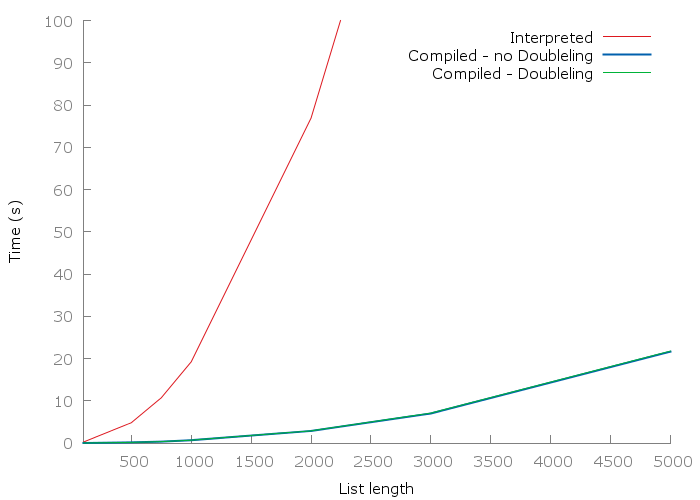
\includegraphics[width=0.7\textwidth]{quicksort.png}
  \caption{Quicksort}
\end{figure}

The performance when compiling is impressive here. The time is divided by around 20. The complexity in $O(n^2)$ was expected since a sorted list is the worst case of the quicksort algorithm. 

Performances are nearly identical with or without doubling.

\begin{figure}[!htbp]
  \centering
  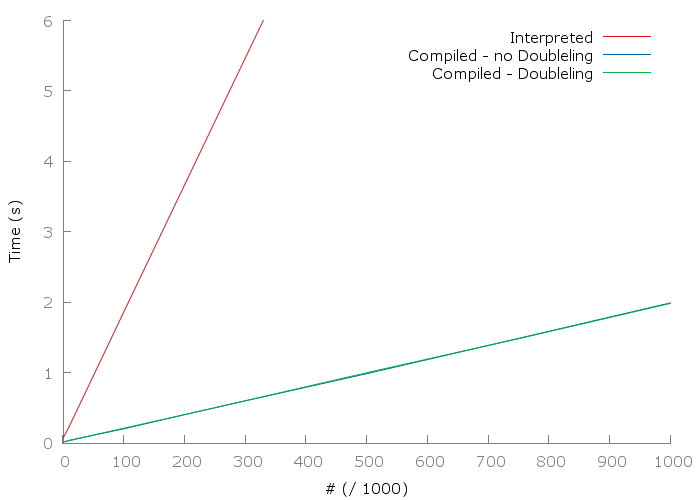
\includegraphics[width=0.7\textwidth]{sumlist.png}
  \caption{Sum over list}
\end{figure}

We get similar result here: Compiled programs are far faster than evaluated ones, around 10 times faster. Doubling and Splicing do not change anything to performances.

\begin{figure}[!htbp]
  \centering
  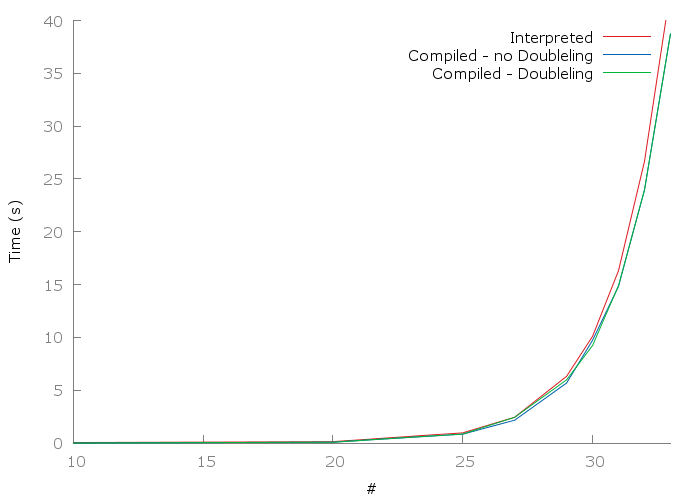
\includegraphics[width=0.7\textwidth]{fib.png}
  \caption{Fibonacci}
\end{figure}

Performances are very bad on the naive Fibonacci program: the compiled program is as slow as the interpreted one. This is a bit surprising and show the fact that the compiler is not really doing any optimization work, on the contrary. 

I think the explication is the following: a function is boxed and unboxed every time it's called. Since this program main computation is to make a lot of functions call, the compiled program is very slow to run.

This could be easily improved by boxing things in a smarter way.

Again, Doubling and Splicing do not change anything to this.\\

Whereas some problems remain unsolved in the compiler, results are positive: Doubling and Splicing actually do not change performances. 

We can note that, as opposed to what we could expect, binary files are not significantly bigger; but an example could probably be found where the file is far larger with Doubling. The ocaml compilation time is also around 10\% longer.

\subsection{Programs with queries}

The only way to actually test queries alone is to fire queries as fast as possible, so a simple test has been done here: repeating the hello example presented in \refsec{intro:query} 10000 times and compare the results. 

The query server was running on the same computer than the program to eliminate network delay. The processor was multicore, so the presence of the server should not affect too much the performances of the program.

The interpreter is running in 5.98s and the compiled file in 3.18s. The gain is around 47\%. The CPU occupation show us that both times, the database server was kept busy by the requests but it was kept busier (the CPU occupation was two times higher) when the compiled file was running. So even when the querying time is limiting performances, the compiled program is significantly faster than the interpreted one. 

\section{Conclusion}

The existing compiler for \links was extended to support querying, using the theory behind the translation from an effect based language to a quotation based language. This extension does not affect performances of programs without queries and show better performances than the interpreter for programs with queries.

However, there is a lot of improvement than can still be made:
\begin{itemize}
\item Apply Doubling only when needed or make the doubling compatible with a dead code elimination procedure;
\item Avoid passing the pair of functions when only one of them is needed;
\item Found a way to make the application of the Splicing operator verified by \ocaml's typechecker. This could probably be possible by using the boxed values type in a clever way. Some attempt has be made on this aspect, but only unsuccessfully for now.
\item Make \links back-end more modular and avoid the duplication of functionality.
\end{itemize}\ 

This internship gave me an opportunity to have a closer look at how a compiler is working in details. This has been very instructive in many ways. This also show me how challenging it can be to mix external elements into the functional paradigm. It is definitely an exciting approach I will keep following.



\newpage

\begin{thebibliography}{99}
\bibitem{links:tiers} \href{http://groups.inf.ed.ac.uk/links/papers/links-fmco06.pdf}{Links: web programming without tiers}: Ezra Cooper, Sam Lindley, Philip Wadler and Jeremy Yallop. FMCO 2006
\bibitem{links:formlets} \href{http://groups.inf.ed.ac.uk/links/papers/formlets-essence.pdf}{The essence of form abstraction}: Ezra Cooper, Sam Lindley, Philip Wadler and Jeremy Yallop. APLAS 2008
\bibitem{links:effect} \href{http://homepages.inf.ed.ac.uk/slindley/papers/corelinks.pdf}{Row-based effect types for database integration}: Sam Lindley and James Cheney. TLDI 2012
\bibitem{links:comp} \href{http://groups.inf.ed.ac.uk/links/papers/undergrads/steven.pdf}{Compiling Links server-side code}: Steven Holmes. BSc honors thesis, University of Edinburgh
\bibitem{links:querycomp} Effective Quotation: James Cheney, Sam Lindley and Philip Wadler. Draft
\bibitem{links:querynorm} The Script-Writer's Dream: How to Write Great SQL 
in Your Own Language, and Be Sure It Will Succeed. Ezra Cooper. DBPL 2009.
\bibitem{linq} LINQ: reconciling object, relations and XML in the .NET framework. Erik Meijer, Brian Beckman, Gavin M. Bierman. SIGMOD Conference 2006
\end{thebibliography}

\section*{Annex}

\subsection*{The targeted \ocaml subset\label{ocamlsubset}}
\begin{lstlisting}[language={[Objective]Caml}]
type code =
  | Unit | Bool of bool | Int of num | Char of char | NativeString of string | Float of float
  | Var of string
  | Rec of (string * string list * code) list * code
  | Fun of string list * code 
  | Let of string * code * code
  | If of (code * code * code)
  | Call of (code * code list)
  | Pair of code * code
  | Triple of code * code * code
  | Lst of code list
  | Case of code * ((code * code) list) * ((code * code) option)
  | Table of code * code * (string * base_type) list
  | Tail of code
\end{lstlisting}

\end{document}
